\part{Analysing data}
\frame{\partpage}

%\begin{frame}
%	\begin{center}
%		
\includegraphics[height=0.9\textheight]{science_bitch}
%	\end{center}
%\end{frame}

\begin{frame}{The scientific method}
	\begin{center}
		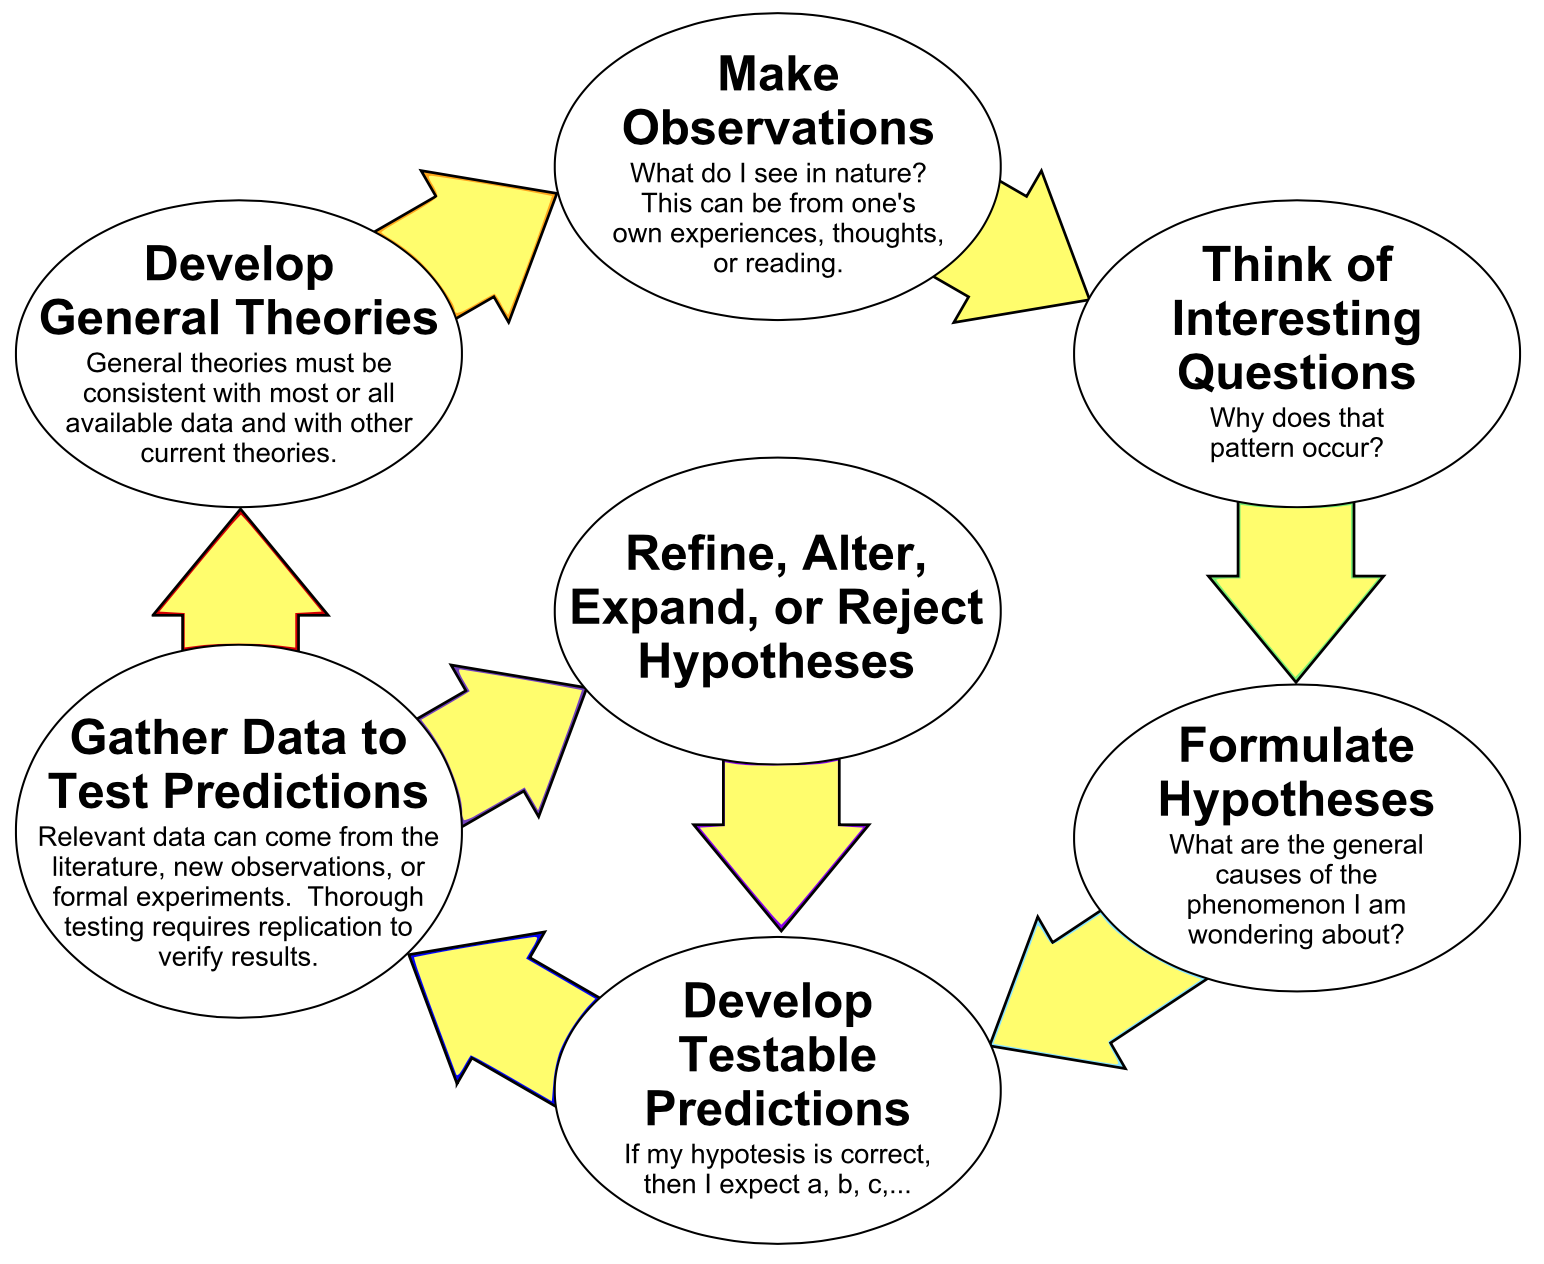
\includegraphics[width=0.8\textwidth]{scientific_method}
	\end{center}
\end{frame}

\begin{frame}{Statistical significance}
	\pause Is a D6 biased if...
	\begin{itemize}
		\pause\item You roll it once and it comes up a six?
		\pause\item You roll it 3 times and it comes up a six twice?
		\pause\item You roll it 60 times and it comes up a six 59 times?
		\pause\item You roll it 60 times and it comes up a six 11 times?
		\pause\item You roll it 600 times and it comes up a six 110 times?
		\pause\item You roll it 6,000,000 times and it comes up a six 1,100,000 times?
	\end{itemize}
\end{frame}

\begin{frame}{Statistical significance}
	\begin{itemize}
		\pause\item Every statistical result has a non-zero probability of being a \textbf{coincidence}
		\pause\item Know your \textbf{confidence intervals}
		\pause\item Beware of \textbf{$p$-value fishing}
	\end{itemize}
\end{frame}

\begin{frame}
	\begin{center}
		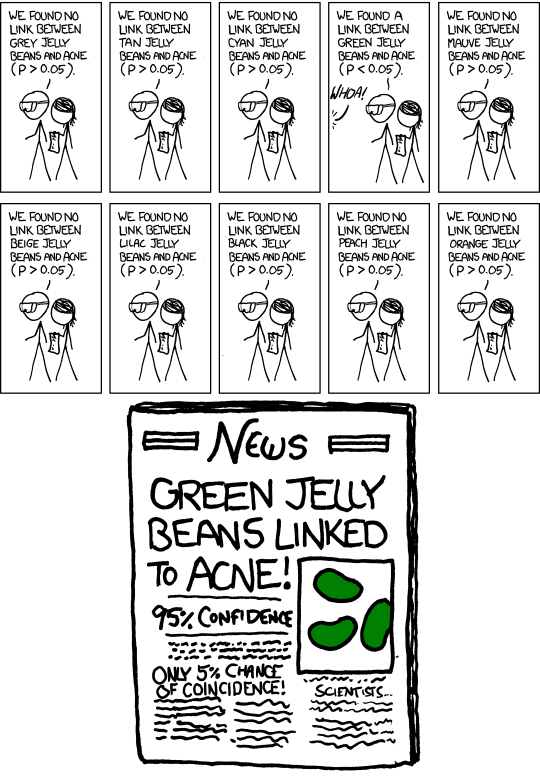
\includegraphics[height=0.9\textheight]{xkcd_significant_crop}
	\end{center}	
\end{frame}

\begin{frame}{Statistical significance vs effect size}
	\begin{itemize}
		\pause\item High statistical significance does not always mean large \textbf{effect size}
		\pause\item E.g.\ red team wins 5,010,000 matches out of 10,000,000
		\pause\item This is statistically significant, but only a 0.1\% effect size
	\end{itemize}
\end{frame}

\begin{frame}{Correlation does not imply causation}
	\pause
	\begin{center}
		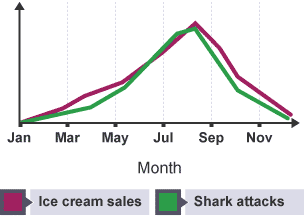
\includegraphics[height=0.5\textheight]{shark_attacks}
	\end{center}
\end{frame}

\begin{frame}{Correlation does not imply causation}
	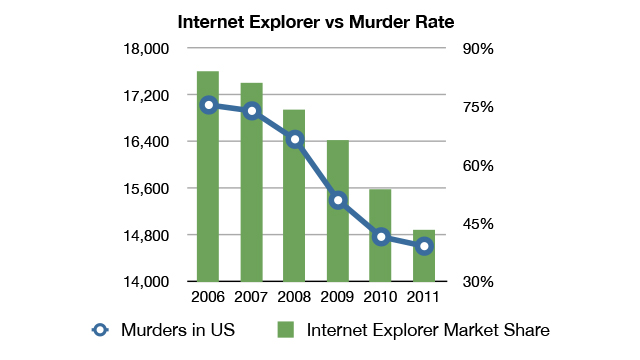
\includegraphics[width=\textwidth]{internet_explorer_murder_rate}
\end{frame}
